\section{Aufgabenstellung}\label{Aufgabenstellung}
In diesem Projekt sollen gegebene Agilent-Logdateien geparst werden. Aus den geparsten Zeilen soll ein Baum in einem Intermediate-Format erstellt werden. Der erzeugte Baum wird im Hauptspeicher des Rechners gehalten. Die Weiterverarbeitung des Baumes im Intermediate-Format erfolgt in einem anderen Projekt und ist nicht Gegenstand dieser Arbeit. In diesem Projekt muss das Intermediate-Format nicht entworfen werden. Statt dessen wird es von Felix Deutschmann und Daniel Horbach �bernommen. Das Intermediate-Format ist unter 

https://github.com/sifedeut/agilentCompiler.git 

zu finden. Ein Baum im Intermediate-Format wird immer nur aus einer Agilent-Logdatei erzeugt, d.h. es soll nicht ein Baum aus zwei oder mehreren Agilent-Logdateien erzeugt werden.

Das Frontend soll nur Knotennamen ber�cksichtigen, die in den zur Verf�gung stehenden Agilent-Logdateien auch vorkommen. Andere Knotennamen brauchen im Frontend nicht implementiert werden. Treten bei der Verarbeitung einer Agilent-Logdatei einmal unerwartete Knotennamen auf, werden diese in der Datei UnsupportedNodes.txt weggeschrieben.

Die Reihenfolge der Kindknoten spielt bei der Erstellung des Baumes keine Rolle.

In Abbildung \ref{fig:Zwischenformat} auf Seite \pageref{fig:Zwischenformat} ist f�r die folgende Agilent-Logdatei das Zwischenformat vereinfacht dargestellt.

\begin{verbatim*}
{@BATCH|SEP13676|E|12|1||btest|120828133549||venture1|SEP13676|RevA|||
{@BTEST|VM122691746|00|120828133615|000046|0|all||n|n|120828133701||1
{@BLOCK|f1%jp1_2|00
{@A-JUM|1|+3.197647E+00{@LIM2|+1.130000E+00|+0.000000E+00}}
}
{@PF|pins|0|0
}
{@BLOCK|f2%jp1_2|00
{@A-JUM|2|+3.200943E+00{@LIM2|+2.130000E+00|+0.000000E+00}}
}
{@BLOCK|f3%jp1_2|00
{@A-JUM|3|+3.169900E+00{@LIM2|+3.130000E+00|+0.000000E+00}}
}
}
}
\end{verbatim*}

\begin{figure}[htp]
\centering
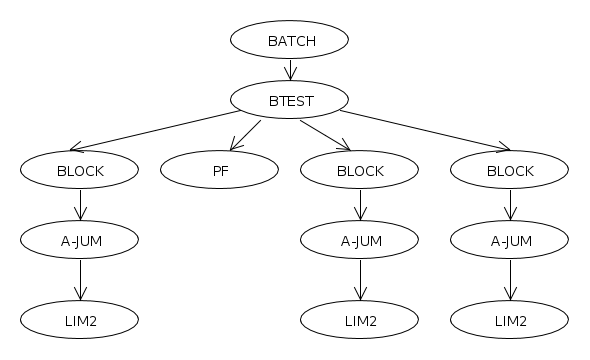
\includegraphics[width=0.8\textwidth]{Ingo/Bilder/Baum.png}
\caption{vereinfachte Darstellung des Zwischenformates}
\label{fig:Zwischenformat}
\end{figure}